\subsection{Comparision algorithm}
For comparing values of two word processor we just need to do a simple XOR operation. If we apply XOR on two word processor in fact we are comparing two words bit by bit and the result would be another word processor having 0 if two bits in the same position matched otherwise it's 1. In VHD each bit is coding one character in a read. Thus, our XOR result shows how many of \emph{base pairs (bp)} between two strings matched (0s) and how many didn't match (1s).
Since we are coding our base pairs with three bits, we should do XOR for each level separately and then accumulate our final result with applying OR operation  on all results. With this approach our final result would be a word processor which each of its bit will tell us whether two \textit{bp}s from two different strings matched or not. Next step would be computing number of miss matches between two strings. Since we have segmented our string into multiple segments for the last step we need to sum up each segment's result and then compare it with the user defined threshold \textit{e}. Figure \ref{fig:fig3} shows following procedure.
  
\begin{figure}
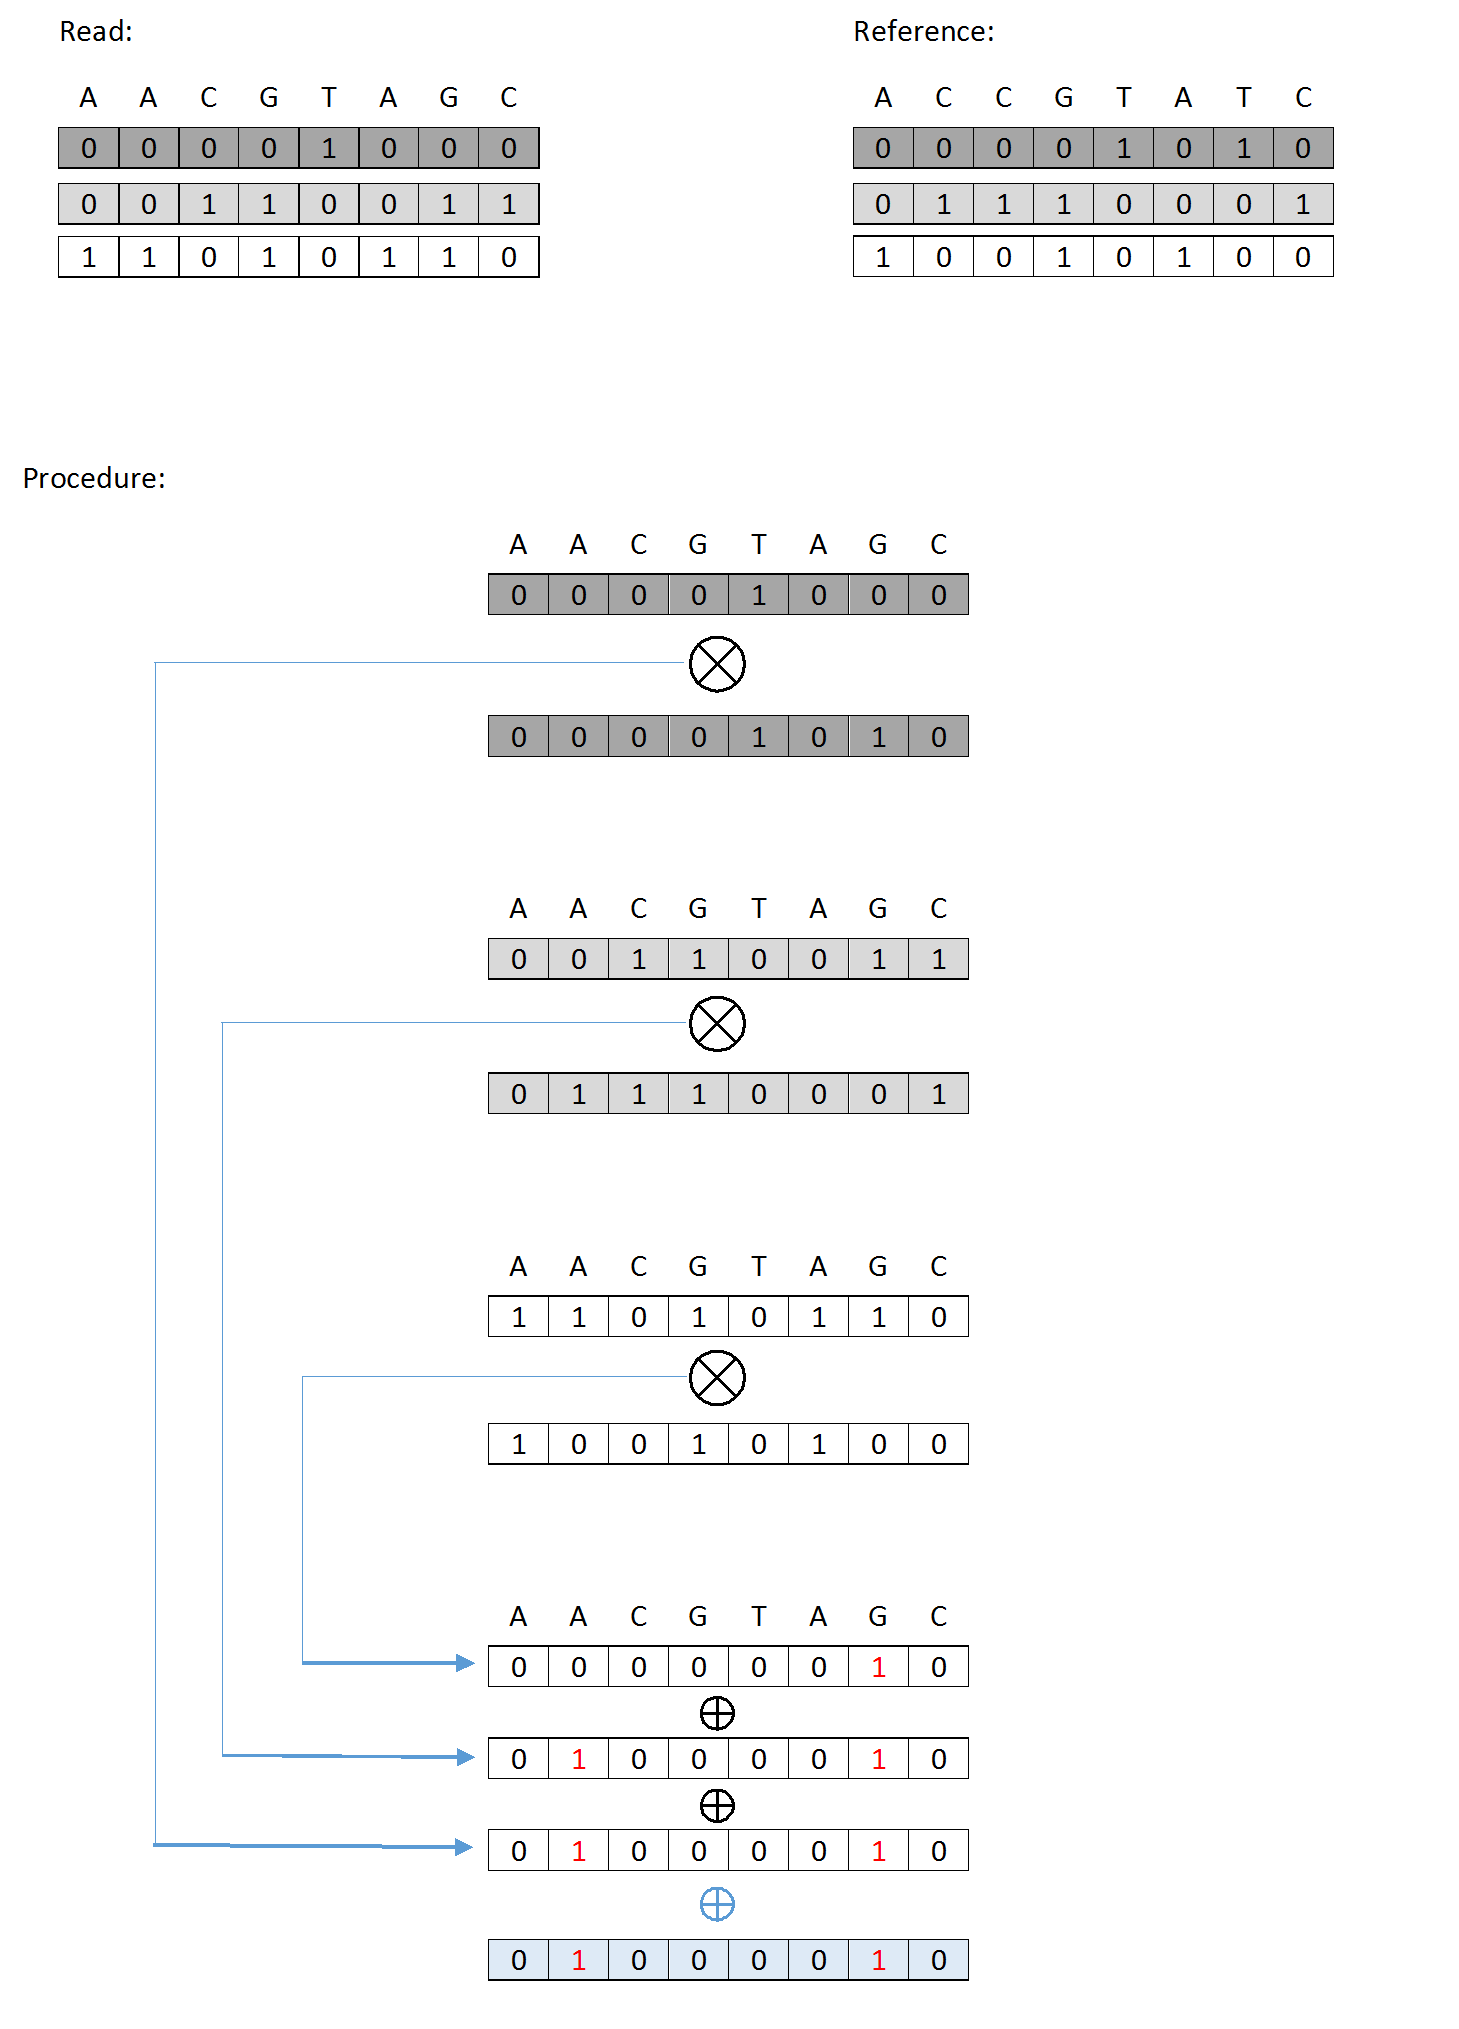
\includegraphics[\width=\linewidth]{figures/Untitled2.png}
\end{figure}

\subsection{Filtering}
As we mentioned in the introduction part user defined error threshold is between $0\%$ and $5\%$ of mappings length and read's length is usually between 80 till 120 bps which means our error threshold won't be bigger than 5 or 6 errors and as a result nearly $98\%$ of our mappings would be incorrect. These numbers show that if we don't filter out our data approximately $98\%$ of our computation would be useless. 

First step for filtering out our data is to computing number of errors and comparing it with \emph{e} for each segment. Instead of summing up segment's results and do comparision with \emph{e} in the last step we can compare each segment's result with \emph{e} sepratly. Therefore, we are doing more operations for correct reads since instead of counting number of ones in the result vector once and then compare it with the error threshold we are counting number of ones per each segment and then compare it with error thershold.  But the point is we are doing these additional computations for just $2\%$ of our total reads and for the rest of the reads we are saving instructions because now per each segment we can decide that whether we have passed error threshold or not and if yes we can stop comparision operation for that read and start comparing next read with our reference. Now base on our word processor's length (\emph{w}) and our read's length (\emph{l}) we can compute number of operations we are doing for each read.

\begin{equation}
\nonumber
n_{operations} = n_{XOR} + n_{OR} + n_{popcnt} + n_{gt} \\


n_{segments} =  \lceil \frac{l}{w} \rceil \\


n_{XOR} = n_{segments} \times (k-1) \\


n_{OR} = n_{segments} \times (k-1) \\


n_{popcnt} = n_{gt} = n_{segment} \\

\end{equation}  
  
Now number of operations we are doing to comparing reads with a reference would be depend on the size of our word processor. In modern CPUs $w$ is usually 32 or 64 (and if we use SIMD operations our register's length can be 128 or more). For instance if our word processor length is equal to 64 and our read's length is 100 then first segment would contain $64\%$ of our read. In other words we still using big portion of reads to determine should we continue our comparison procedure or should we stop since even in the first $64\%$ number of errors exceed \emph{e}. According to Figure ... using first $64\%$ of each reads can filter out nearly .... of our data with comparing just first segment.\\
But what if we can answer this question with even less comparison. For instance what if we use only first 16 bps of our read and compare it with the reference. Figure ... shows that number of reads going to filter won't change significantly and the number would stay the same. However, if we use first 16bps we will have more segments and as a result number of operation we should do for rest of our reads will increase but since we can filter out more data it will still have positive effect on our performance.\\
Now if we get same result from comparing 16 first bits in compare with first 32 bits then we can reduce number of bits transferring with just using 16 bits. Suppose our word processor length is equal to 32s but we just need 16 bits, as a result we are not using 16bits of our processor. But we can increase instruction level parallelism with interleaving different reads and instead of loading one read into each word processor we can now load two reads and process them together. Consequitively, our parallelism will limit to our word processor length. If we can provide bigger processor word (like SIMD registers) we can process more reads in a same time. Figure ... is the modified schema for comparing multiple reads with one reference. \\
  
\subsection{Computing Stride} \label{stride}
Using first 16 bits of a read and putting multiple reads in a one word processor even though it increases data level parallelism of our output but now for each we need to figure out which one is a valid read and which one is not. In addition, even if we could figure out valid and non-valid reads from each other we will have memory fragmentation issue. Since we are not fetching our data consecutively and sometime we need to skip part of the memory. In this section we will describe our solutions for these two problem.\\
First, to figure out valid reads we can use a secondary secondary data. For each read we use one flag bit telling current situation of the read and each time when we finish comparing, for instance, 16 bits of all reads we recompute flag bit to see whether the read is still valid. Figure ... shows added step to our previous algorithm.\\

Flag bits tell us what are the next reads we are going to copy to our word processor. There are two ways to fetch data into processor word, one way is each time when we are feeling the processor word first we can check flag of the read and decided whether we should copy it to our word processor or check the next flag. But then we have to do at least one additional comparing operation to decide. Another way is pre-computing reads we need to fetch. Suppose, we have stored reads in our memory and we just now beginning address of the reads in the memory. We need additional information about our data so that we can load them into our word processor without checking flags. We know that we are going to fetch 16 bits for each read but the problem is that we don't know where should we begin. Using flags in our previous part we can compute addresses we need to load our data from the memory. We use Fibonaci algorithm to compute distances from beginning address. Later, for loading data into our processor we just add distances to our beginning address and load correct data into our word processor. We called these distances \emph{Strides}. Using strides helps us to not checking flags each time we are trying to load our data and we just need to check flags once.

\subsection{Coding}
In this section we talk about coding schema and its role in our algorithm. In our storage layout we describe how we are saving our data in vertical fashion. But how we can interpret this layout and use it to improve our performance.\\
In storage layout we suggest to use below coding:\\
 IMAGE, IMAGE, IMAGE
 
If we just look at highest bit of the characters in this coding we have:

IMAGE

Thus we can recognize T out of other three characters A, C, G with looking at only their highest bit, since T is the only character which its highest bit is 1. The same would happen in their middle bits. Because of our coding schema we can recognize C and G out of A and T. Since, C and G's middle bit is 1 but A and T's middle bit is 0.\\
Base on above observation and our algorithm we can infer an important point. With suggested coding schema at first step (comparing highest bits) we are able to recognizing all substitution of T with A, C and G with only comparing highest bit of our character. In fact, our final output for highest bit is an vector of 0s and 1s which telling us at which location substitution of T with A, C and G have been happened.

 
  
  
  
  
  